% -*-LaTeX-*-

\section{Evaluation}
\label{sec:eval}

% Focus on the evaluation of libpfs : is it really local speed
% Evaluation of PFSD depends on the technology that is intended to be used
% libpfs evaluation :
%    eval tech details / env
%    benchmark : LFS + small Write (relinking + meta_data updt) overhead
%    Faster than NFS_local : Definitely usable. 
%    Propagation happens asynchronously
%    without the user knowing + sequentially
% pfsd evaluation :
%    successful setup of personal cloud
%    network usage especially on WAN still an issue
%    Hidden Costs :
%      Log size -> pruned
%      Deleted Files -> Ficus deleted files gargabe collection algorithm
% Global evaluation :
%    it's cool, but definitely not designed to scale <-> pClouds

\subsection{libpfs}

This section presents an evaluation of pFS local performance. Our goal
is to show that, locally, pFS provides a seamless user experience,
updates being propagated ayncrhonously. We compare the performances of
pFS, ext3, Fuse only (We implemented a trivial Fuse based file system
replicating all calls directly to the local file system), and NFS
(Protocol v.3 over LAN with default settings) over a set of
microbenchmarks. The machine used is a 2.4 GHz Dual-Core Intel Xeon,
with 2GB of RAM and a Gibabit ethernet controller, running Ubuntu
Server 8.04 distribution. The microbenchmarks we used are the ones
used for the evaluation of LFS~\cite{rosenblum:lfs}. The small file
benchmark (LFS\_S, Figure \ref{LfsS}) consists of the creation of
10,000 small (4096 bytes) files (LFS\_SC) in 100 different
directories, the access for reading of those files (LFS\_SR), and
finally their deletion (LFS\_SD). We augmented the small file
benchmark with a small file write benchmark (LFS\_SW), which opens
every file for writing, truncates it, rewrites the 4096 bytes and
calls {\tt fsync}.  We added this benchmark to illustrate the case
where libpfs incurs the most overhead (extra {\tt link} operation
for versioning, and cache flushing when syncing to disk), as
described in section \ref{sec:impl}. The large file benchmark (LFS\_L,
Firgure \ref{LfsL}) consists of writing sequentially 30,000 blocks of
4096 bytes (LFS\_LSW), reading them sequentially (LFS\_LSR),
re-writing them randomly (LFS\_LRW) and finally re-reading them
randomly (LFS\_LRR).

\begin{figure}[ht]
\begin{center}
  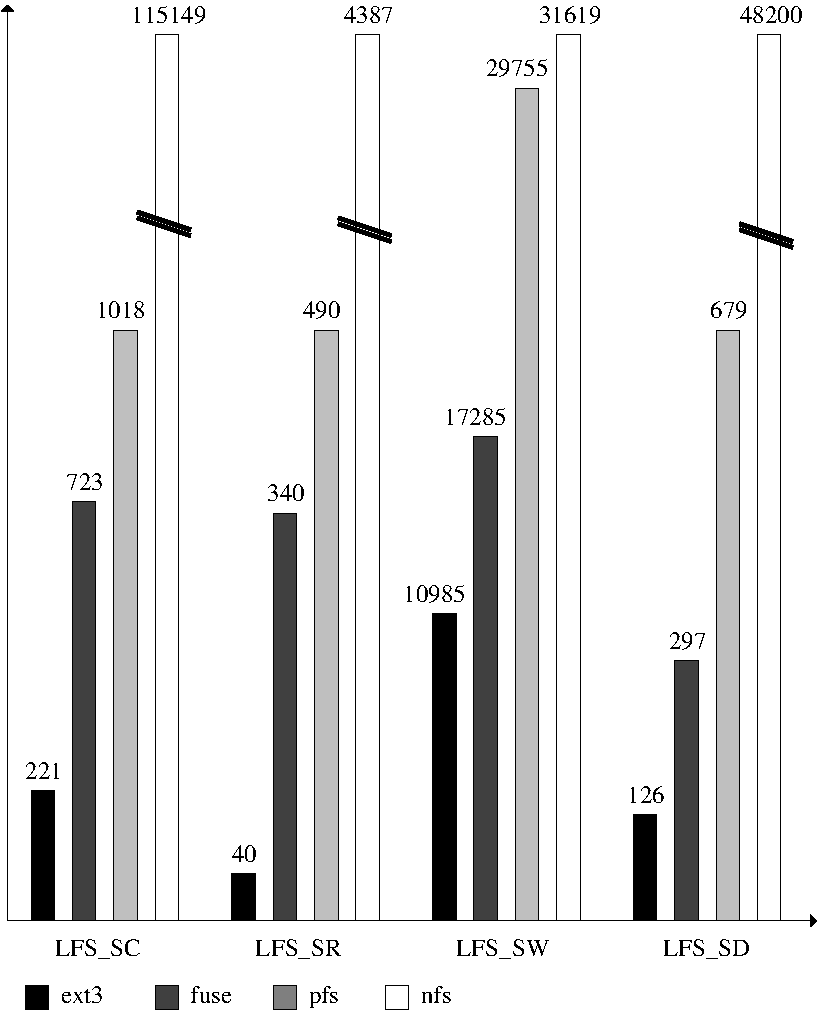
\includegraphics [scale=0.55] {lfs_s}
  \caption{\label{LfsS}
    {\small LFS\_S benchmark : creation (LFS\_SC), reading (LFS\_SR),
      writing (LFS\_SW) and deletion (LFS\_SD) of 10,000 small files
      in 100 directories. All values are in ms.}}
\end{center}
\end{figure}


\begin{figure}[ht]
\begin{center}
  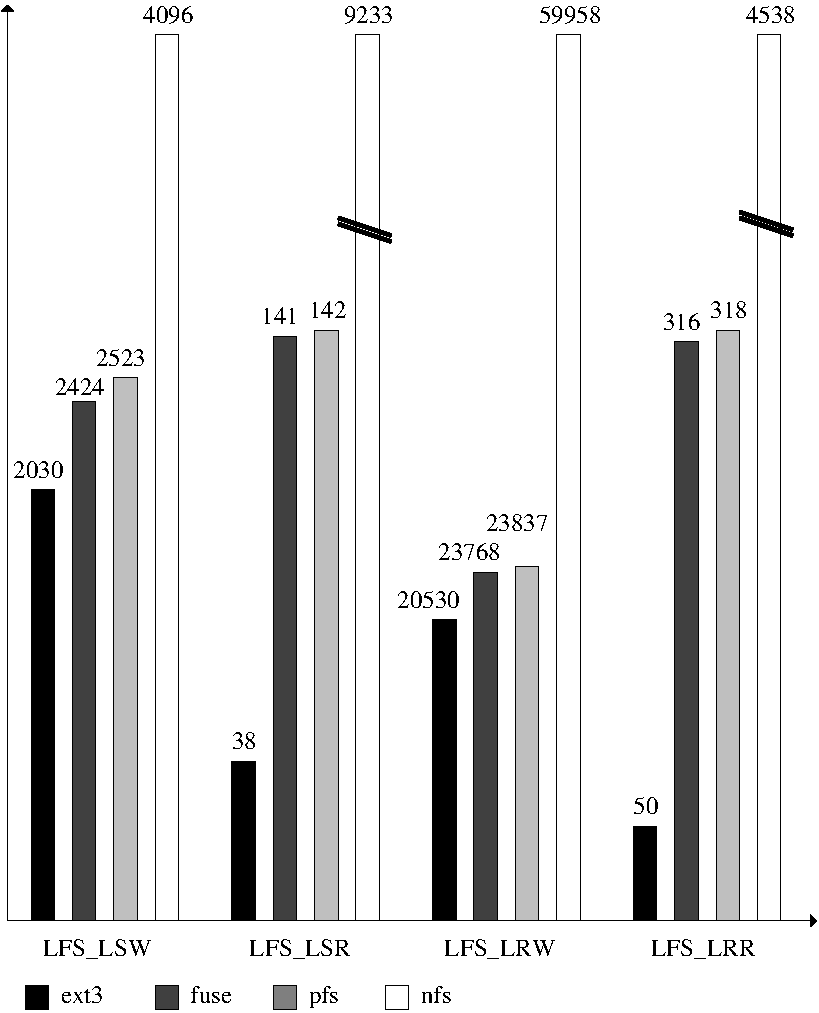
\includegraphics [scale=0.55] {lfs_l}
  \caption{\label{LfsL}
    {\small LFS\_L benchmark : senquential writing (LFS\_LSW),
      sequential reading (LFS\_LSR), random writing (LFS\_LRW), random
      reading (LFS\_LRR) of a large file. All values are in ms.}}
\end{center}
\end{figure}

\begin{figure*}[ht]
\begin{center}
  \begin{tabular}[t]{|r|c|c|c|c|c|}
    \hline
    & \emph{untar} & \emph{configure} & \emph{compile} 
    & \emph{clean} & \emph{end-to-end} \\
    \hline

    \textbf{ext3} & 11.0  & 333.5 & 562.8 & 4.6  & 911.8  \\
    \textbf{pFS}  & 33.2  & 351.9 & 581.1 & 10.6 & 976.9  \\
    \textbf{NFS}  & 167.8 & 662.1 & 826.0 & 66.1 & 1722.1 \\
    \hline
  \end{tabular}
\end{center}
\caption{Macrobenchmarks. untar, configure, compile and clean of
  gzip-1.2.4. All values are in ms.}
\label{fig:macrobench}
\end{figure*}

The benchmarks are synthetic, and do not represent realistic
workloads. The goal is to show the strengths and weaknesses of
libpfs. Figure \ref{LfsL} shows, as expected, that versioning
maintenance does not incur any visible overhead compared to Fuse for
large files. pFS is substantially faster than NFS on every benchmark
except the small write benchmark (Figure \ref{LfsS}). This benchmark
emphasizes the operation that incurs the most overhead due to
versionning maintenance: pFS performs comparatively to NFS on this
benchmark where it is three times slower than native ext3.

Figure \ref{fig:macrobench} shows the performance of pFS (in the same
conditions as previously) on a macrobenchmark consisting of untaring,
configuring, compiling and cleaning gzip-1.2.4. pFS incurs a 7\%
overhead over ext3 (while NFS incurs a 88\% overhead) on the
end-to-end execution which shows that pFS local performances are
perfectly acceptable for day-to-day computing.

\subsection{pfsd}

In this section we evaluate the bandwidth consumption of pFS and the
overhead due to the propagation of the versioning information. We
sequentially runned the LFS\_SC, LFS\_SR, LFS\_SW, and LFS\_SD
microbenchmarks and mesured the bandwidth usage they incurred on
an NFS client, and a pFS \emph{replica} participating in a \emph{file
  system} with only one other device.
\footnote{Disclaimer : we used the kernel driver byte count to
  evaluate the bandwidth consumption. The results may contain noise
  that we tried to limit as much as possible (results issued from a
  more controlled experiment will be available in a near future).}

\begin{figure}[ht]
\begin{center}
  \includegraphics [scale=0.77] {bandw}
  \caption{\label{Bandw}
    {\small Bandwidth usage.}}
\end{center}
\end{figure}

Figure \ref{Bandw} shows that the simplicity of our prototype's protocol
incurs a limited overhead to the actual size of the 10.000 files
(cumulating a total 39 MB). pfsd retransmits the whole content of
every file during the LFS\_SW benchmark, which could be drastically
optimized, especially since LFS\_SW rewrites the same content as
LFS\_SC. The total bandwidth usage is slightly higher for the LFS\_SC
benchmark, due to the 100 directories creation wich totalizes
aproximatively 50 KB of bandwidth consumption. Obviously, if the
updates where to be propagated to more than one device, those number
would be accordinlgy demultiplied. This experiment illustrates the
fact that the versioning information generated by pFS does not incur a
large overhead compared to NFS, even when updating a large number of
small files.

Even if our prototype of pfsd is not yet optimized for bandwitdth
consumption, it already allowed us to experience the benefits of our
serverless personal cloud model and the ease of use of libpfs'
versioning system. WAN and LAN communications over IP being achieved
at virtually no cost, pfsd opportunistically communicates updates
resulting in an efficient propagation of the state among the
devices. pFS is transparent to use, does not require any maintenance
once the devices are configured, and conflicts rarely occur on a
relatively well connected set of devices. We believe that it would be
really difficult to create conflicts if cell phones and media players
were to be used as simple relays, even with a small capacity and a
simple LRU cache for updates.

\subsection{Hidden Costs}

There are a few hidden costs associated with the use of pFS. First, the
update log used by pfsd : even if they are deleted once propagated to
every devices or superseded, this log may grow considerably should a
device remain unused for a long period of time without being removed
from the system. ``Rumor Mongering'' technique as described
in~\cite{demers:epidemic} could be used to alleviate this issue.

Second, libpfs keeps track of deleted files to avoid ambiguity in face
of resources creation and removal. Such deleted entries are only kept
for directories that are still accessible on a replica which limits
their number. Nevertheless, such entries can be garbage collected. A
solution to this issue has already been provided in~\cite{page:ficus}
under the section : ``Insert/Delete ambiguity''.

\endinput


% Local Variables:
% tex-main-file: "main.ltx"
% tex-command: "make;:"
% tex-dvi-view-command: "make preview;:"
% End:
